%
% $Id: SANDExampleReportstrict.tex,v 1.21 2006/10/04 00:32:14 rolf Exp $
%
% This is an example LaTeX file which uses the SANDreport class file.
% It shows how a SAND report should be formatted, what sections and
% elements it should contain, and how to use the SANDreport class.
% It uses the LaTeX report class and the strict option.
%
% Get the latest version of the class file and more at
%    http://www.cs.sandia.gov/~rolf/SANDreport
%
% This file and the SANDreport.cls file are based on information
% contained in "Guide to Preparing {SAND} Reports", Sand98-0730, edited
% by Tamara K. Locke, and the newer "Guide to Preparing SAND Reports and
% Other Communication Products", SAND2002-2068P.
% Please send corrections and suggestions for improvements to
% Rolf Riesen, Org. 9223, MS 1110, rolf@cs.sandia.gov
%
% \documentclass[pdf,ps2pdf,12pt,report,strict]{SANDreport}
\documentclass[12pt]{SANDreport}
\usepackage{moreverb}
\usepackage{epsfig}
\usepackage{amsfonts}
\usepackage[boxed]{algorithm2e}
% \usepackage{graphicx}
\usepackage{mathptmx}	% Use the Postscript Times font
\usepackage[FIGBOTCAP,normal,bf,tight]{subfigure}

% \usepackage[light]{draftcopy}
% \draftcopyName{\today - DRAFT}{60}

% If you want to relax some of the SAND98-0730 requirements, use the "relax"
% option. It adds spaces and boldface in the table of contents, and does not
% force the page layout sizes.
% e.g. \documentclass[relax,12pt]{SANDreport}
%
% You can also use the "strict" option, which applies even more of the
% SAND98-0730 guidelines. It gets rid of section numbers which are often
% useful; e.g. \documentclass[strict]{SANDreport}


% ---------------------------------------------------------------------------- %
%
% Set the title, author, and date
%
\title{Trilinos ThreadPool Library v1.1}

\author{H. Carter Edwards \\
	hcedwar@sandia.gov \\
	Computational Simulation Infrastructure \\
	Sandia National Laboratories\\
	P.O. Box 5800\\
	Albuquerque, NM 87185 \\
}

    % There is a "Printed" date on the title page of a SAND report, so
    % the generic \date should generally be empty.
    \date{}


% ---------------------------------------------------------------------------- %
% Set some things we need for SAND reports. These are mandatory
%
\SANDnum{SAND2009-8196}
\SANDprintDate{December 2009}
\SANDauthor{H. Carter Edwards}

% ---------------------------------------------------------------------------- %
% Include the markings required for your SAND report. The default is "Unlimited
% Release". You may have to edit the file included here, or create your own
% (see the examples provided).
%
% \include{MarkUR} % Not needed for unlimted release reports


% ---------------------------------------------------------------------------- %
% The following definition does not have a default value and will not
% print anything, if not defined
%
% \SANDsupersed{SAND1901-0001}{January 1901}
% ---------------------------------------------------------------------------- %
% New commands

\newenvironment{blist}%
  {\begin{list}{$\bullet$}{\setlength{\topsep}{0.5ex} \setlength{\itemsep}{0.5ex}\setlength{\parsep}{0pt}}}%
  {\end{list}}

\newcommand{\itemB}{\item[$\bullet$]}

\newcommand{\arrowlabel}[1]{\stackrel{\mbox{\scriptsize \it #1}}{\longrightarrow}}

% ---------------------------------------------------------------------------- %
%
% Start the document
%
\begin{document}
\maketitle

% ------------------------------------------------------------------------ %
% An Abstract is required for SAND reports
%
\begin{abstract}
\vspace{-1em}
%
A ``manycore revolution'' is underway in high performance computing (HPC) to move from model of interconnected single-core nodes with a single thread of execution to many-core nodes with many threads execution 
\cite{SciDAC:ManycoreRevolution:WebSite}. 
%
This revolution leaves HPC application programmers with the challenge of maximizing parallel performance at both the interconnect level (\emph{i.e.} process parallelism) and the manycore level (\emph{i.e.} thread parallelism).
%
The ThreadPool library has been developed within the Trilinos Project \cite{Trilinos:ACM} to provide HPC applications with a simple interface to make effective use of thread parallelism on CPU-based manycore nodes.
%
\end{abstract}

% ------------------------------------------------------------------------ %
% An Acknowledgement section is optional but important, if someone made
% contributions or helped beyond the normal part of a work assignment.
% Use \section* since we don't want it in the table of context
%
%\clearpage
%\chapter*{Acknowledgment}

% ------------------------------------------------------------------------ %
% The table of contents and list of figures and tables
% Comment out \listoffigures and \listoftables if there are no
% figures or tables. Make sure this starts on an odd numbered page
%
\cleardoublepage		% TOC needs to start on an odd page
\tableofcontents
\listoffigures
\listofalgorithms
% \listoftables

% ---------------------------------------------------------------------- %
% An optional preface or Foreword
%\clearpage
%\chapter*{Preface}
%\addcontentsline{toc}{chapter}{Preface}

% ---------------------------------------------------------------------- %
% An optional executive summary
%\clearpage
%\chapter*{Summary}
%\addcontentsline{toc}{chapter}{Summary}

% ---------------------------------------------------------------------- %
% An optional glossary. We don't want it to be numbered
%\clearpage
%\chapter*{Nomenclature}
%\addcontentsline{toc}{chapter}{Nomenclature}
%\begin{description}
%\item[*]
%\end{description}

% ---------------------------------------------------------------------- %
% This is where the body of the report begins; usually with an Introduction
%
\SANDmain		% Start the main part of the report

\section{Introduction}

A ``manycore revolution'' is underway in high performance computing (HPC) to move from model of interconnected single-core nodes with a single thread of execution to many-core nodes with many threads execution 
\cite{SciDAC:ManycoreRevolution:WebSite}. 
%
This revolution leaves HPC application programmers with the challenge of maximizing parallel performance at both the interconnect level (\emph{i.e.} process parallelism) and the manycore level (\emph{i.e.} thread parallelism).
%
The ThreadPool library has been developed within the Trilinos Project 
\cite{Trilinos:WebSite} to provide HPC applications with a simple interface to make effective use of thread parallelism on CPU-based manycore nodes.


Parallelism at the interconnect level is being effectively exploited by HPC applications, with the Message Passing Interface (MPI) \cite{MPI:Standard:WebSite} as the \emph{de-facto} programming model.
%
Research is in progress to effectively exploit parallelism at the manycore level.
%
The architecture of the HPC node drives manycore programming models in two directions: homogeneous thread parallelism versus heterogeneous thread parallelism.
%
In homonegenous manycore parallelism all processing cores of a node are equivalent---they have equal capabilities and access to the node's resources 
(\emph{e.g.}, memory, interconnect, disks).
%
In heterogeneous manycore parallelism the processing cores residing within a node have different compute capabilities and different means of accessing the node's resources.


Homogeneous manycore and heterogeneous manycore programming models have fundamental differences; however, an HPC application can adopt the layered software architecture illustrated in Figure~\ref{fig:HybridParallelArchitecture} to isolate these differences as much as feasible.
%
\begin{figure}[h]
\begin{center}
\includegraphics[viewport=0.5in 0.75in 3in 4.5in,angle=0,scale=1]{HybridParallelLayers.eps}
\caption{Software layers for the separation of concerns within HPC applications exploiting both distributed and manycore parallelism}
\label{fig:HybridParallelArchitecture}
\end{center}
\end{figure}
%
The primary objective of this layered software architecture is to separate concerns such that porting or refactoring one layer (\emph{e.g.}, manycore parallelism) has minimal impact on the remaining layers.
%
In this architecture the lowest-level computational kernels are \emph{stateless} functions that perform their computations on data provided through the manycore resource management layer.


A primary function of the intra-node (manycore) resource management layer is to dispatch the stateless computational kernels to be called in parallel on each available thread.
%
This is the intended functionality of the ThreadPool library, as well as other libraries and programming languages.
%
A well-known library supporting homogeneous manycore parallelism is the Intel Threading Building Blocks (TBB) \cite{TBB:Book}, which provides a C++ interface to manage thread-parallel execution of C++ functions.
%
A well-known language supporting heterogeneous manycore parallelism is 
CUDA \cite{CUDA:WebSite}, 
which supports thread-parallel execution of functions written in the CUDA language on GPGPU manycores manufactured by 
NVIDIA \cite{NVIDIA:Website}.


The ThreadPool library provides a simple, minimalistic, and highly portable package with which HPC applications can effectively exploit homogeneous manycore parallelism; and through which the performance implications of this architectural layer can be easily explored.
%
It is written in the standard C programming language and utilizes a small portion of the standard \textbf{pthreads} \cite{pthreads:Standard} in Linux environments.
%
This report describes the application programmer interface (API) and performance of the ThreadPool library available through the Trilinos project \cite{Trilinos:WebSite}. 



\section{Application Programmer Interface (API)}

The ThreadPool manages a set of parallel threads running on the local computational node and sharing the resources of that computational node.
%
An application can dispatch thread-parallel work, defined by a work subprogram and work information, to the ThreadPool.
%
The ThreadPool causes each parallel thread, including the application's \emph{main} thread, to call the application's work subprogram with the application's work information.
%
The ThreadPool application programmer interface (API), ThreadPool implementation, and application's work subprograms conform to the standard C programming language.


The ThreadPool has four states: NULL, BLOCKED, READY, and ACTIVE.
%
These states and state transitions are illustrated in the ThreadPool state diagram given in Figure~\ref{fig:ThreadPoolStates}.
%
Each state transition occurs through application calls to the ThreadPool functions noted in Figure~\ref{fig:ThreadPoolStates}.
%
\begin{figure}[h]
\begin{center}
\fbox{
\includegraphics[viewport=0.5in 0.5in 2.75in 4.75in,angle=270,scale=1]{StateDiagram.eps}
}
\caption{ThreadPool state diagram with state transitions identified by thread pool functions}
\label{fig:ThreadPoolStates}
\end{center}
\end{figure}

The ThreadPool is in the ACTIVE state while running an application's work subprogram.
%
A work subprogram may be run in several different thread-parallel modes, 
as described in Sections~\ref{sec:RunWork}-\ref{sec:WorkSubprogramWithReduce}.
%
An application selects the thread-parallel mode by calling the associated version of a 
\texttt{TPI\_Run\_*} function.


\clearpage
\subsection{Initialization, Finalization, and Blocking}

\subsubsection{TPI\_Init( int thread\_count )}

The ThreadPool starts in the NULL state, without any additional threads of execution.
%
An application calls the \texttt{TPI\_Init} function to create \texttt{thread\_count-1} threads and transition the ThreadPool from the NULL state to the READY state.
%
This \texttt{TPI\_Init} function can only be called when the ThreadPool is in the NULL state.
%
These created threads are in addition to the application's \emph{main} thread, for a total of 
\texttt{thread\_count} available threads of execution.
%
While in the READY state the ThreadPool is ready to dispatch work routine to threads.


Thread creation and initialization is a time consuming operation.
%
As such the ThreadPool creates threads during initialization and then holds them in the READY state for subsequent use by the application.
%
Threads in the READY state are continually running on the manycore CPU and polling the ThreadPool for work to be performed.
%
This strategy minimizes the time required to dispatch work to threads by maintaining the threads in this \emph{ready to run} state.


It is recommended that the number of requested threads, \texttt{thread\_count}, be no greater than the number of available processing cores.
%
If more threads are requested then the threads will be required to block and unblock 
(\emph{i.e.}, context switch) in order for all of the threads to execute.
%
This blocking and unblocking introduces overhead which degrades thread-parallel performance.


\subsubsection{TPI\_Finalize()}

While in the READY state an application calls \texttt{TPI\_Finalize} to destroy the created threads and transition the ThreadPool to the NULL state.
%
A call to \texttt{TPI\_Finalize} can be followed by a call to \texttt{TPI\_Init} to reinitialize the ThreadPool with a different number of threads.


\subsubsection{TPI\_Block() and TPI\_Unblock()}

While in the READY state the created threads are running and consuming CPU resources.
%
If an application creates additional non-ThreadPool threads, either explicitly or through a different parallel threading library, the ThreadPool threads in the READY state will continually compete with those non-ThreadPool threads for CPU resources.
%
An application may block the ThreadPool created threads to preempt this competition for CPU resources.
%
The \texttt{TPI\_Block()} blocks the ThreadPool created threads and transitions the ThreadPool from the READY state to the BLOCKED state.


An application unblocks the ThreadPool created threads by calling \texttt{TPI\_Unblock()}.
%
This function returns the ThreadPool to the READY state with the ThreadPool created threads running and polling the ThreadPool for work.
%
Blocking and unblocking created threads is a time consuming operation; however, it is not as time consuming as destruction and creation of threads.


\subsubsection{Intended Use}

An application code initializes the ThreadPool, calls a sequence of algorithms, and then finalizes the ThreadPool.
%
An algorithm is assumed to run many thread-parallel computational kernels through a single threading mechanism; \emph{e.g.}, ThreadPool, OpenMP, or TBB.
%
An algorithm which runs computational kernels through the ThreadPool mechanism would unblock the worker threads, run its sequence of thread-parallel computational kernels, and then return the worker threads to the blocked state.
%
This assumed application and algorithm flow is summarized in Figure~\ref{fig:WorkFlow}.

\begin{figure}[h]
\center
\small 
\begin{boxedverbatim}
#include<TPI.h>

int main(...)
{
  TPI_Init( thread_count );
  /* 
   *  Application's program control flow
   *  calls application's algorithms. 
   */
  TPI_Finalize();
}

void an_application_algorithm(...)
{
  const int was_blocked = TPI_Isblocked();
  if ( was_blocked ) TPI_Unblock();
  /* 
   *  Run many thread-parallel computational kernels... 
   */
  if ( was_blocked ) TPI_Block();
  return ;
}
\end{boxedverbatim}
\caption{Assumed work flow for an application and its algorithms}
\label{fig:WorkFlow}
\end{figure}


%--------------------------------------------------------------------------------
\clearpage
\subsection{Running Work Subprograms} \label{sec:RunWork}

While in the READY state an application calls one of the \texttt{TPI\_Run} functions to dispatch  work subprograms to be called on all available threads, including the application's main thread.
%
A \texttt{TPI\_Run} function can only be called when the ThreadPool is in the READY state.
%
While an application's work subprogram is running the ThreadPool is in the ACTIVE state.
%
When all invocations of the work subprogram return, the ThreadPool returns to the READY state.



\subsubsection{Work Subprogram}

An application's work subprogram is called by the ThreadPool an application-specified number of times.
%
Each call to the work subprogram is responsible for performing an application-specified portion of the computational work.
%
Two pieces of information is required by a call to the work subprogram:
(1) the computational work to be performed and
(2) a means of partitioning this work.


An application's work subprogram is a function conforming to the C language interface defined in Figure~\ref{fig:WorkSubprogram}.
%
A work subprogram determines which portion of work that it should perform from members of the input 
\texttt{TPI\_Work\_Struct} argument.
%
\begin{figure}[h]
\center
\small
\begin{boxedverbatim}
struct TPI_Work_Struct {
  const void * info ;       /**< Shared info input to TPI_Run         */
  void       * reduce ;     /**< Data for reduce operation, if any    */
  int          count ;      /**< Count of work requested via TPI_Run  */
  int          rank ;       /**< Rank  of work for the current call   */
  int          lock_count ; /**< Count of locks requested via TPI_Run */
};

typedef const struct TPI_Work_Struct TPI_Work ;

typedef void (*TPI_work_subprogram)( TPI_Work * work );
\end{boxedverbatim}
\caption{TPI work subprogram C language interface defined in the \texttt{TPI.h} header file}
\label{fig:WorkSubprogram}
\end{figure}
%
\begin{blist}
\item The \texttt{work->info} member provides a pointer to application-provided work information.  This work information is shared by all calls to a work subprogram on all threads.  It is declared constant to promote safe multi-threaded access.
%
\item The \texttt{work->count} member identifies the total number times the work subprogram is being called during a single call to a \texttt{TPI\_Run} function.
%
\item The \texttt{work->rank} member is given a unique value for each call of the work subprogram.  These values are in the range \mbox{[0..\texttt{work->count}-1]}.  
Due to non-determinism of thread-execution there is no guaranteed correlation between the 
\texttt{work->rank} value and the calling order of the work subprogram.
These \texttt{work->rank} and \texttt{work->count} members provide the minimal information required for a call to a work subprogram to determine its portion of the total work to be performed.
%
\end{blist}
%
The remaining \texttt{TPI\_Work\_Struct} members are described with respect to the calling \texttt{TPI\_Run} functions.

\clearpage
\subsubsection{Calling Work Subprograms via TPI\_Run\_threads(\ldots)}

\begin{center}
\small
\begin{boxedverbatim}
int TPI_Run_threads( TPI_work_subprogram work_subprogram  ,
                     const void *        work_info ,
                     int                 lock_count /* = 0 */ );
\end{boxedverbatim}
\end{center}

The \texttt{TPI\_Run\_threads} function is used to call an application's work subprogram 
once on each available thread, both main and created threads.
%
A simple use of this function to perform a thread-parallel \mbox{$Y=\alpha*X+Y$} operation is illustrated in Figure~\ref{fig:WorkSubprogramAXPY}.

\begin{figure}[h]
\small
\center
\begin{boxedverbatim}
typedef struct {
  int n ;
  double a ;
  double * x ;
  double * y ;
} WorkInfo ;

void daxpy( int n , double a , double * x , double * y )
{
  WorkInfo work_info = { n , a , x , y };
  TPI_Run_threads( tpi_daxpy , & work_info , 0 );
}
void tpi_daxpy( TPI_Work * work )
{
  const WorkInfo * const info = (const WorkInfo *) work->info ;
  int begin , end , i ;
  compute_span_of_work( work->count , work->rank , info->n , & begin , & end );
  for ( i = begin ; i < end ; ++i ) { 
    work->y[i] += work->a * work->x[i] ; 
  }
}
\end{boxedverbatim}
\caption{Example implementation of a simple, thread parallel AXPY operation using \texttt{TPI\_Run\_threads}}
\label{fig:WorkSubprogramAXPY}
\end{figure}


When the application's work subprogram is called by each thread the \texttt{TPI\_Work} argument (see Figure~\ref{fig:WorkSubprogram}) is populated with the following information.
%
\begin{blist}
\item \texttt{work->info} = pointer to \texttt{work\_info} --- the application-supplied \emph{shared} work data, 
\item \texttt{work->count} = the total number of threads calling the work subprogram, and
\item \texttt{work->rank} = the rank of the calling thread.
\end{blist}

\clearpage
\subsubsection{Calling Work Subprograms via TPI\_Run(\ldots)}

\begin{center}
\small
\begin{boxedverbatim}
int TPI_Run( TPI_work_subprogram work_subprogram  ,
             const void *        work_info ,
             int                 work_count  ,
             int                 lock_count /* = 0 */ );
\end{boxedverbatim}
\end{center}

An application can specify that the work subprogram is called \texttt{work\_count} times, regardless of the number of available threads.
%
The ThreadPool threads use an internally-shared work counter to guarantee the correct number of calls, and to provide a unique \texttt{work->rank} for each call.
%
In this interface the \texttt{TPI\_Work\_Struct} is populated with the following information.
%
\begin{blist}
\item \texttt{work->info} = pointer to \texttt{work\_info} --- the application's \emph{shared} work data, 
\item \texttt{work->count} = \texttt{work\_count} --- the specified number of calls to the work subprogram, and
\item \texttt{work->rank} = the rank of the call out of the specified number of calls.
\end{blist}



This interface is intended for applications that 
(1) have a large amount of work to perform and
(2) have units of work with an irregular computational load.
%
In this situation the application can partition its irregular work into many more units of work that there are threads, and then dispatch the work subprogram to process these \texttt{work\_count} units of work.
%
As each thread completes a call to the application's work subprogram it will claim the next unit of work from the shared work counter.


This interface provides an application with a means for automatically (but only approximately) balancing computational work among threads.
%
The quality of this load balancing is dependent upon the the variability of the work load among the units of work. 


\subsection{Running Work Subprograms with Locks} \label{sec:RunWorkLock}

When a work subprogram updates a shared variable or data structure that update must be thread safe.
%
One strategy for thread safe updates is with \emph{mutually exclusive locks} 
(referred to as \emph{mutex} in the \textbf{pthreads} API).
%
Locks provide mutually exclusive execution of those portions of a work subprogram that access a shared variable or data structure that is updated by the work subprogram.
%
This usage is illustrated by the simple, thread-parallel implementation of a dot product given in Figure~\ref{fig:WorkSubprogramDDOTlocking}.

\begin{figure}[h]
\small
\center
\begin{boxedverbatim}
typedef struct {
  int n ;
  double * result_pointer ;
  const double * x ;
  const double * y ;
} WorkInfo ;

double ddot( int n , const double * x , const double * y )
{
  double result = 0.0 ;
  WorkInfo work_info = { n , & result , x , y };
  TPI_Run_threads( tpi_ddot , & work_info , 1 /* lock_count */ );
  return result ;
}
void tpi_ddot( TPI_Work * work )
{
  const WorkInfo * const info = (const WorkInfo *) work->info ;
  double local_result = 0.0 ;
  int begin , end , i ;
  compute_span_of_work( work->count , work->rank , info->n , & begin , & end );
  for ( i = begin ; i < end ; ++i ) { 
    local_result += work->y[i] * work->x[i] ; 
  }
  TPI_Lock(0);                              /* probable blocking */
  *(work->result_pointer) += local_result ; /* serialized */
  TPI_Unlock(0);
}
\end{boxedverbatim}
\caption{Example implementation for a simple, thread parallel DDOT operation using \texttt{TPI\_Run\_threads}, \texttt{TPI\_Lock}, and \texttt{TPI\_Unlock}}
\label{fig:WorkSubprogramDDOTlocking}
\end{figure}

In the illustrative implementation (Figure~\ref{fig:WorkSubprogramDDOTlocking}), each thread-parallel call to \texttt{tpi\_ddot} has its own thread-local accumulation variable \texttt{local\_result}.
%
Summation of the local accumulation into the global accumulation is thread safe by the calls to \texttt{TPI\_Lock} and \texttt{TPI\_Unlock}.
%
The first thread to arrive at \texttt{TPI\_Lock} acquires the mutually exclusive lock and proceeds with the local-to-global accumulation.
%
If a second thread arrives at this function call it will block and wait for the first thread to release the lock via \texttt{TPI\_Unlock}.
%
Once the first thread releases the lock the second thread unblocks, acquires the lock, and proceeds with its own contribution to the summation.


Using mutually exclusive locks has the performance liabilities of 
\begin{blist}
\item serializing thread execution between \texttt{TPI\_Lock} and \texttt{TPI\_Unlock},
\item introducing overhead for blocking and unblocking threads, and
\item introducing a non-deterministic race condition for the local-to-global accumulation.
\end{blist}
%
The serialization and overhead liabilities increase execution time.
%
The non-deterministic liability can cause computions to be non-repeatable.
%
All of these liabilities can be addressed for reduction operations through the following section.


\clearpage
\subsection{Running Work Subprograms with Reductions} \label{sec:WorkSubprogramWithReduce}

Alternate versions of the \texttt{TPI\_Run} and \texttt{TPI\_Run\_threads} functions,
\texttt{TPI\_Run\_reduce} and \texttt{TPI\_Run\_threads\_reduce} respectively,
are defined to support efficient reduction operations.
%
An example usage of this reduction-supporting interface is given in 
Figure~\ref{fig:WorkSubprogramDDOTreduce}.

\begin{center}
\small
\begin{boxedverbatim}
typedef void (*TPI_reduce_init)( TPI_Work * work );
typedef void (*TPI_reduce_join)( TPI_Work * work , const void * reduce );

int TPI_Run_threads_reduce( TPI_work_subprogram work_subprogram  ,
                            const void *        work_info ,
                            TPI_Reduce_join     reduce_join ,
                            TPI_Reduce_init     reduce_init ,
                            int                 reduce_size ,
                            void *              reduce_data );

int TPI_Run_reduce( TPI_work_subprogram work_subprogram  ,
                    const void *        work_info ,
                    int                 work_count  ,
                    TPI_Reduce_join     reduce_join ,
                    TPI_Reduce_init     reduce_init ,
                    int                 reduce_size ,
                    void *              reduce_data );
\end{boxedverbatim}
\end{center}

\paragraph{\texttt{work->reduce}:}
%
Each call to the \texttt{work\_subprogram} accumulates its portion of the reduction operation into a reduction variable, pointed to by the \texttt{work->reduce} argument.
%
Each call to the \texttt{work\_subprogram} has exclusive access to the reduction variable --- no locking is required.
%
Exclusive access is guaranteed by each thread having its own copy of the reduction variable.
%
This copy is allocated to be \texttt{reduce\_size} bytes and is initialized by a call to the application-provided \texttt{reduce\_init} function. 


\paragraph{\texttt{reduce\_join}:}
%
As threads complete their calls to the \texttt{work\_subprogram} the per-thread reduction variables are reduced (joined together) via the application's \texttt{reduce\_join} function.
%
The final result is reduced into the application-provided reduction variable pointed to by the \texttt{reduce\_data} argument.
%
These join operations occur without additional serialization, without extra runtime overhead, and are deterministic.
%
Thus for algorithms with reduction operations, or with updates to shared variables which can be expressed as reduction operations, this interface resolves the performance liabilities of the locking / unlocking approach. 



\begin{figure}[ht]
\small
\center
\begin{boxedverbatim}
typedef struct {
  int n ;
  const double * x ;
  const double * y ;
} WorkInfo ;

double ddot( int n , const double * x , const double * y )
{
  double result = 0.0 ;
  WorkInfo work_info = { n , & result , x , y };
  TPI_Run_threads_reduce( tpi_ddot , & work_info , 
                          tpi_ddot_join , tpi_ddot_init ,
                          sizeof(result) , & result );
  return result ;
}
void tpi_ddot( TPI_Work * work )
{
  const WorkInfo * const info = (const WorkInfo *) work->info ;
  double * const local_result = (double*) work->result ;
  int begin , end , i ;
  compute_span_of_work( work->count , work->rank , info->n , & begin , & end );
  for ( i = begin ; i < end ; ++i ) { 
    *local_result += work->y[i] * work->x[i] ; 
  }
}
void tpi_ddot_join( TPI_Work * work , const void * reduce )
{ *((double*) work->reduce) += *((const double*) reduce); }

void tpi_ddot_init( TPI_Work * work }
{ *((double*) work->reduce) = 0 ; }
\end{boxedverbatim}
\caption{Example implementation of a simple, thread parallel DDOT operation using \texttt{TPI\_Run\_threads\_reduce}}
\label{fig:WorkSubprogramDDOTreduce}
\end{figure}



\section{Performance Considerations}

The ThreadPool manages a set of parallel \emph{pthreads} \cite{pthreads:Standard} to run on a CPU-multicore node.
%
The purpose of these threads is to support thread-parallel execution of 
\emph{high performance computing} (HPC) work subprograms.
%
As such the implementation of the ThreadPool addresses the following potential performance impediments.
%
\begin{blist}
\item  The time required to create and destroy threads.
\item  The time required to block and unblock threads.
\item  Sharing CPU resources with threads that exist outside of the ThreadPool.
\item  Serialization of code segments within the HPC kernel.
\end{blist}



\subsection{Pool of Threads}

The ThreadPool creates a pool of threads at initialization, holds them ready to execute HPC work subprograms, and terminates the threads only upon request
(Figure~\ref{fig:ThreadPoolStates}).
%
It is intended for the HPC application to initialized the ThreadPool when it begins execution and terminate the ThreadPool only after all of the application's work has been completed.
%
This \emph{thread pool} strategy pays the time-cost of creating and deleting threads only once.



\subsection{Ready, Spinning Threads}

A thread is either running or blocked on the compute node.
%
When a thread is running 
(1) it is assigned to a CPU-core and
(2) its instructions and data are present in the nodes' main memory and cache memory; within limitations of the node's capacity and operating system kernel.
%
When a thread is blocked its instructions and data may be ejected from cache memory or even swapped out of main memory.
%
Activating a blocked thread can include time-costs of
(1) reassigning the thread to a CPU-core,
(2) reloading its instructions and data into main memory and cache memory.


The time-cost of unblocking a blocked thread is minimized by keeping threads actively running on the CPU-cores, even when they are doing no work.
%
\emph{Spinning} is the term associated with threads which are actively running and waiting for work.
%
When the ThreadPool is in the READY state (Figure~\ref{fig:ThreadPoolStates}) the created threads are spinning.
%
When an application calls one of the \texttt{TPI\_Run} functions the ThreadPool attaches the application's work subprogram and work information to each thread, and these threads then call the work subprogram in thread-parallel.


\subsection{Blocking Threads}

An application may utilize multiple thread-parallel capabilities such as this ThreadPool,
OpenMP \cite{OpenMP:Website}, 
Intel threading builing blocks (TBB) \cite{TBB:Book}, or 
Boost's C++ thread pool \cite{boost:threadpool}.
%
If the ThreadPool created threads are spinning in the READY state then these threads will compete with other thread-parallel capabilities for CPU resources.
%
As such the ThreadPool provides an application with a means of blocking and unblocking ThreadPool created threads.
%
As previously noted, a blocked thread is detached from a CPU core and may have its instruction and data ejected from cache or entirely swapped out of main memory.



\subsection{Work Completion and Reductions}

Every call to a \texttt{TPI\_Run} function waits for all created threads to return to the READY state before returning to the application.
%
This completion operation is a parallel collective barrier in which the application's main thread of execution cannot proceed until all created threads have completed.
%
The barrier is a parallel reduction operation with the reduced data being the created threads' transition from the ACTIVE state to the READY state.
%
This reduction is implemented as a fan-in operation with the application's main thread of execution being the root of the fan-in tree.


An application's parallel reduction operations 
(Section~\ref{sec:WorkSubprogramWithReduce})
are attached to the work-completion barrier.
%
This implementation performs the given reduction operation without having to introduce locking or additional synchronizations.
%
Furthermore, the reduction is deterministic due to the deterministic fan-in operation for the work-completion barrier.






\section{Hybrid Parallel Performance}

Runtime performance is investigated through the hybrid parallel implementation of a simple ``mini-application.''
%
This mini-application generates a parallel distributed sparse matrix and then applies conjugate gradient solution algorithm iterations to that system of equations.
%
The sparse matrix is generated from applying a 27-point stencil to a regular three dimensional grid, resulting in 27 non-zero coefficients per matrix row associated with locations in the interior of the grid.
%
The distribution of the sparse matrix is obtained by applying a recursive coordinate bisection \cite{RCB:1989} partitioning to the grid.


Performance is studied by running this mini-application on a hybrid parallel machine.
%
This mini-application is run in the following three modes.
\begin{blist}
\item An all-MPI mode where one MPI process is run on each CPU core.
\item A one-MPI-process-per-node mode where one worker thread is created for each additional CPU core on the node.
\item A one-MPI-process-per-socket mode where one MPI process is run on each CPU socket and one worker thread is created for each additional CPU core on the socket.
\end{blist}


\clearpage
\subsection{Parallel Conjugate Gradient Algorithm Iteration}

A simple conjugate gradient solver algorithm for a sparse linear system of equations is implemented using two-level parallelism: MPI for inter-process parallelism and ThreadPool for intra-process parallelism.
%
This parallel algorithm can be implemented with a small number of basic linear algebra subprogram (BLAS) kernels:
$\mathbf{y}=\mathbf{x}$,
$dot(\mathbf{x},\mathbf{y})$,
$\mathbf{y}=\alpha*\mathbf{x}+\beta*\mathbf{y}$, and
$\mathbf{y}=\mathbf{A}*\mathbf{x}$.
%
For intra-process thread-level parallelism each call to a kernel will have runtime overhead starting and waiting on the local threads.
%
This overhead can be minimized by \emph{fusing} parallel kernels, as presented in Algorithm~\ref{alg:CG-fused}.


\begin{algorithm}[h]
\SetKwInOut{KwInOut}{InOut}
\SetAlgoLined
\DontPrintSemicolon
\Begin(parallel symmetric conjugate gradient algorithm){
\KwIn{$\mathbf{A} \equiv$ sparse symmetric matrix}
\KwIn{$\mathbf{b} \equiv$ right-hand-side vector}
\KwInOut{$\mathbf{x} \equiv$ initial guess, solution vector}
\KwData{$\mathbf{r} \equiv$ residual vector}
\KwData{$\mathbf{p} \equiv$ solution vector update, length = \# columns of $\mathbf{A}$}
\KwData{$\mathbf{Ap} \equiv$ residual vector update}
$\mathbf{r} = \mathbf{b}$ \tcc*{parallel} \;
$\mathbf{p} = \mathbf{x}$ \tcc*{parallel} \;
$\mathbf{Ap} = \mathbf{A} * \mathbf{p}$ \tcc*{parallel} \;
$\mathbf{r} = \mathbf{r} - \mathbf{Ap}$ ; $\delta = dot(\mathbf{r},\mathbf{r})$ \tcc*{fused parallel} \;
$\beta = 0 $ \tcc*{serial} \;
\While(\tcc*[f]{serial}){$\mathit{tolerance} < \delta$ and within iteration limit }{
  $\mathbf{p} = \mathbf{r} + \beta * \mathbf{p}$ \tcc*{parallel} \;
  $\mathbf{Ap} = \mathbf{A} * \mathbf{p}$ ; $\gamma = dot(\mathbf{Ap},\mathbf{p}) $ \tcc*{fused parallel} \;
  $\alpha = \delta / \gamma $ ; $\beta = \delta $ \tcc*{serial} \;
  $\mathbf{x} = \mathbf{x} + \alpha * \mathbf{p}$ ; $\mathbf{r} = \mathbf{r}- \alpha * \mathbf{Ap}$ ; $\delta = dot(\mathbf{r},\mathbf{r})$ \tcc*{fused parallel} \;
  $\beta = \delta / \beta$ \tcc*{serial} \;
}
}
\caption{Conjugate gradient algorithm with \emph{fused} parallel kernels}
\label{alg:CG-fused}
\end{algorithm}


In the conjugate gradient algorithm the matrix vector multiplication step is immediately followed by an inner product of the input and output vectors.
%
Fusing these steps into a single parallel kernel eliminates the thread-wait and thread-start overhead associated with completing the first kernel and starting the second kernel.
%
A thread-parallel work kernel for this operation could separate or fuse these steps.


\clearpage

\subsection{Hybrid Fused Parallel Sparse Matrix Vector Multiplication}

Algorithm~\ref{alg:FusedMXV} describes a hybrid parallel fused implementation of the matrix-vector multiply followed by a dot product of the input and output vectors.
%
In this algorithm the thread work kernel performs both the matrix-vector multiply and the dot product.
%
Internal to the thread work kernel, these two operations can be implemented separate serial linear algebra kernels.


\begin{algorithm}[h]
\SetKwInOut{KwInOut}{InOut}
\SetKwBlock{Call}{Call}{end}
\SetKwBlock{CallThread}{Each thread calls}{end}
\SetKwInOut{KwInOut}{InOut}
\SetAlgoLined
\DontPrintSemicolon
\Begin( Fused parallel function: \mbox{$\gamma = dot( ( \mathbf{y} = \mathbf{A} * \mathbf{x} ) , \mathbf{x} )$}){
\KwIn{$\mathbf{A}_\mathrm{P} \equiv$ this process' rows of matrix $\mathbf{A}$}
\KwInOut{$\mathbf{x}_\mathrm{P} \equiv$ this process' portion of vector $\mathbf{x}$ spans columns of $\mathbf{A}_\mathrm{P}$}
\KwOut{$\mathbf{y}_\mathrm{P} \equiv$ this process' portion of vector $\mathbf{y}$}
\KwOut{$\gamma \equiv$ result of dot product on all processes}
\BlankLine
Gather off-process columns into $\mathbf{x}_\mathrm{P}$ via MPI communication \;
\BlankLine
\Call( \textnormal{TPI\_Run\_threads\_reduce( work\_kernel , reduction\_kernel )}){
\BlankLine
\CallThread( \textnormal{work\_kernel} ){
\KwIn{$\mathbf{A}_\mathrm{P,T} \equiv$ this thread's span of matrix $\mathbf{A}_\mathrm{P}$}
\KwIn{$\mathbf{x}_\mathrm{P} \equiv$ this process' complete input vector}
\KwOut{$\mathbf{y}_\mathrm{P,T} \equiv$ this thread's span of vector $\mathbf{y}_\mathrm{P}$}
\KwOut{$\gamma_\mathrm{T} \equiv$ this thread's contribution to $\gamma$}
\BlankLine
$\mathbf{y}_\mathrm{P,T} = \mathbf{A}_\mathrm{P,T} * \mathbf{x}_\mathrm{P}$ \;
$\gamma_\mathrm{T} = dot( \mathbf{y}_\mathrm{P,T} , \mathbf{x}_\mathrm{P,T} )$ \;
}
\CallThread( \textnormal{reduction\_kernel} ){
\KwInOut{$\gamma_\mathrm{T} \equiv$ this thread's contribution to $\gamma$}
\KwIn{$\gamma_\mathrm{U} \equiv$ another thread's contribution to $\gamma$}
\BlankLine
$\gamma_\mathrm{T} = \gamma_\mathrm{T} + \gamma_\mathrm{U}$ \;
}
}
Reduce $\gamma$ among all processes  via MPI\_Allreduce
}
\caption{Fused hybrid parallel kernel for \mbox{$\gamma = dot( ( \mathbf{y} = \mathbf{A} * \mathbf{x} ) , \mathbf{x} )$} }
\label{alg:FusedMXV}
\end{algorithm}

\clearpage

\subsection{Performance Study}

This performance study was run on an HPC cluster at Sandia National Laboratories.
%
This cluster (called \emph{glory}) consists of 272 quad-socket compute nodes with 2.2 GHz AMD quad-core CPUs, and an Infiniband interconnect.
%
The mini-application was compiled at optimization level 3, using the Intel-11 compiler, OpenMPI, and standard pthreads.


The mini-application is run on 4, 8, 16, and 32 compute nodes with
\begin{blist}
\item one MPI process on each available core,
\item one MPI process on each available socket and worker threads created on each remaining core, and
\item one MPI process on each node and worker threads created on each remaining core.
\end{blist}
%
The compute node architecture provides non-uniform memory access (NUMA) performance between the CPUs and main memory.
%
As such the Linux non-uniform memory access control (numactl) capability is used to attach MPI processes to sockets or cores.



\subsubsection{Processes versus Threads}

Results from the performance studies are summarized in Figures~\ref{fig:CGPerf:np4}-\ref{fig:CGPerf:np32}.
%
Each of these graphs is for a fixed number of compute nodes and thread, where each line is for one of the three approaches to allocating MPI process and pthreads to cores (MPI-per-core, MPI-per-socket,and MPI-per-node).
%
The objective of these studies is to compare the performance of the three MPI process versus pthread allocation approaches over a range of problem sizes.
%
This comparison method is chosen to make apparent the impact of cache memory and non-uniform memory access on performance.


Each graph (Figures~\ref{fig:CGPerf:np4}-\ref{fig:CGPerf:np32}) plots the aggregate gigaflop performance attained from parallel CG iterations over a range of problem size, from less than 1e4 to more than 1e7 grid points (matrix rows).
%
For small problem sizes of less than 1e4 grid points the message passing, thread startup, and thread completion overhead dominates performance --- yielding poor gigaflop performance.
%
From this small problem size, performance of the hybrid parallel approaches improves rapidly with problem size.
%
However, once the matrix and vectors exceeds the CPUs' cache size performance drops significantly and becomes limited by main memory access performance.
%
Furthermore, the performance drop of the MPI-per-node approach is worse due to threads running on four different sockets accessing shared memory allocated physically near its own socket.
%
This is in contrast to the MPI-per-socket and MPI-per-core results where each thread only accesses NUMA memory associated with its own socket.

\clearpage

The approach of using one-MPI-process-per-socket, with one thread per core, consistently yielded the best performance.
%
This result is especially pronounced for the strong scaling (\emph{i.e.}, speed up) results presented in Figures~\ref{fig:CGPerf:scaling1M}~and~\ref{fig:CGPerf:scaling1.7M}.
%
These results are for matrices with 1M and 1.7M rows respectively.

Strong scaling results presented in Figures~\ref{fig:CGPerf:scaling1M}~and~\ref{fig:CGPerf:scaling1.7M} are problem dependent.
%
This dependency is readily apparent in Figure~\ref{fig:CGPerf:scaling} which plots performance versus problem size for each of the one-MPI-process-per-socket test cases.


The following three observations are apparent from these performance results.
\begin{blist}
\item Strong scaling of the one-MPI-process-per-node and one-MPI-process per socket is dramatically better than the one-MPI-process-per-core for small matrices.
\item Performance of the one-MPI-process-per-node mode is significantly worse for large matrices.
\item Performance of the one-MPI-process-per-socket mode is better for (nearly) all sizes of matrices.
\end{blist}
%
Thus for this mini-application running on Sandia's glory cluster, with its NUMA compute nodes, the best performance is achieved with a hybrid parallel strategy of allocating one MPI process to each CPU socket and then applying thread parallelism to utilize the three remaining cores within each socket.
%
The degree to which performance is better depends upon the size and layout of the computational data relative to the CPU cache.
%
If this data can be held in CPU cache for a relatively large number of computations then performance is show to be dramatically better.



\begin{figure}[h]
\center
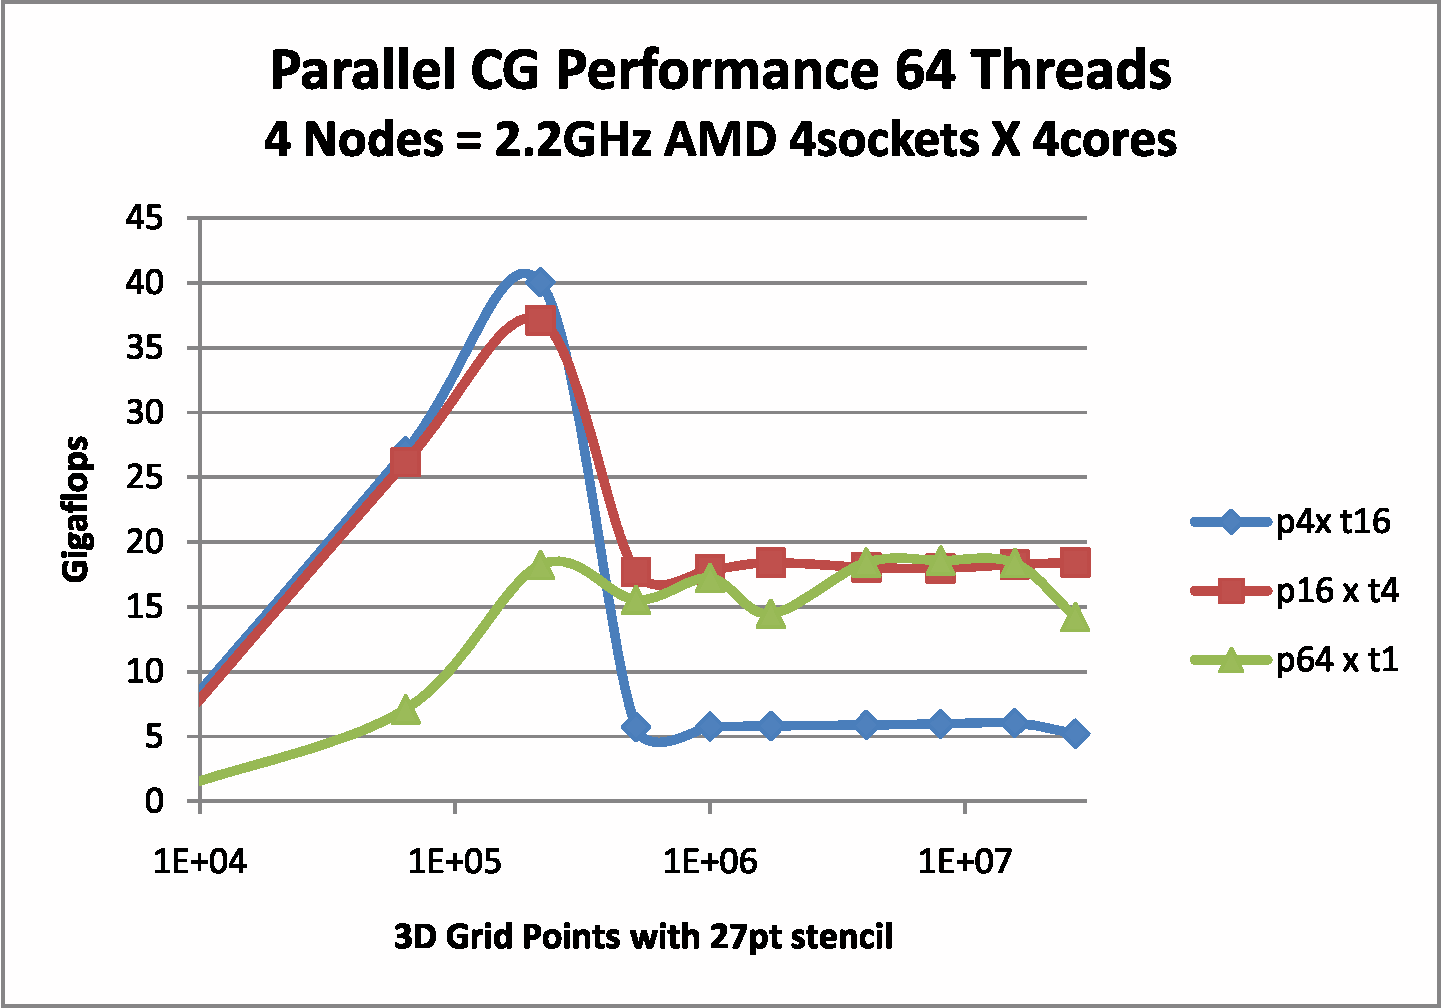
\includegraphics[viewport=1in 0.5in 8.5in 6.5in,angle=0,scale=0.5]{figures/test-hhpccg-intel-11-1-mpi-exe-np4-no-overlap-2}
\caption{Comparison of hybrid parallel conjugate gradient iteration performance for 4 compute nodes with 64 threads: p4 x t16 = one MPI process per node, p16 x t4 = one MPI process per socket, and p64 x t1 = one MPI process per core.}
\label{fig:CGPerf:np4}
\end{figure}

\begin{figure}[h]
\center
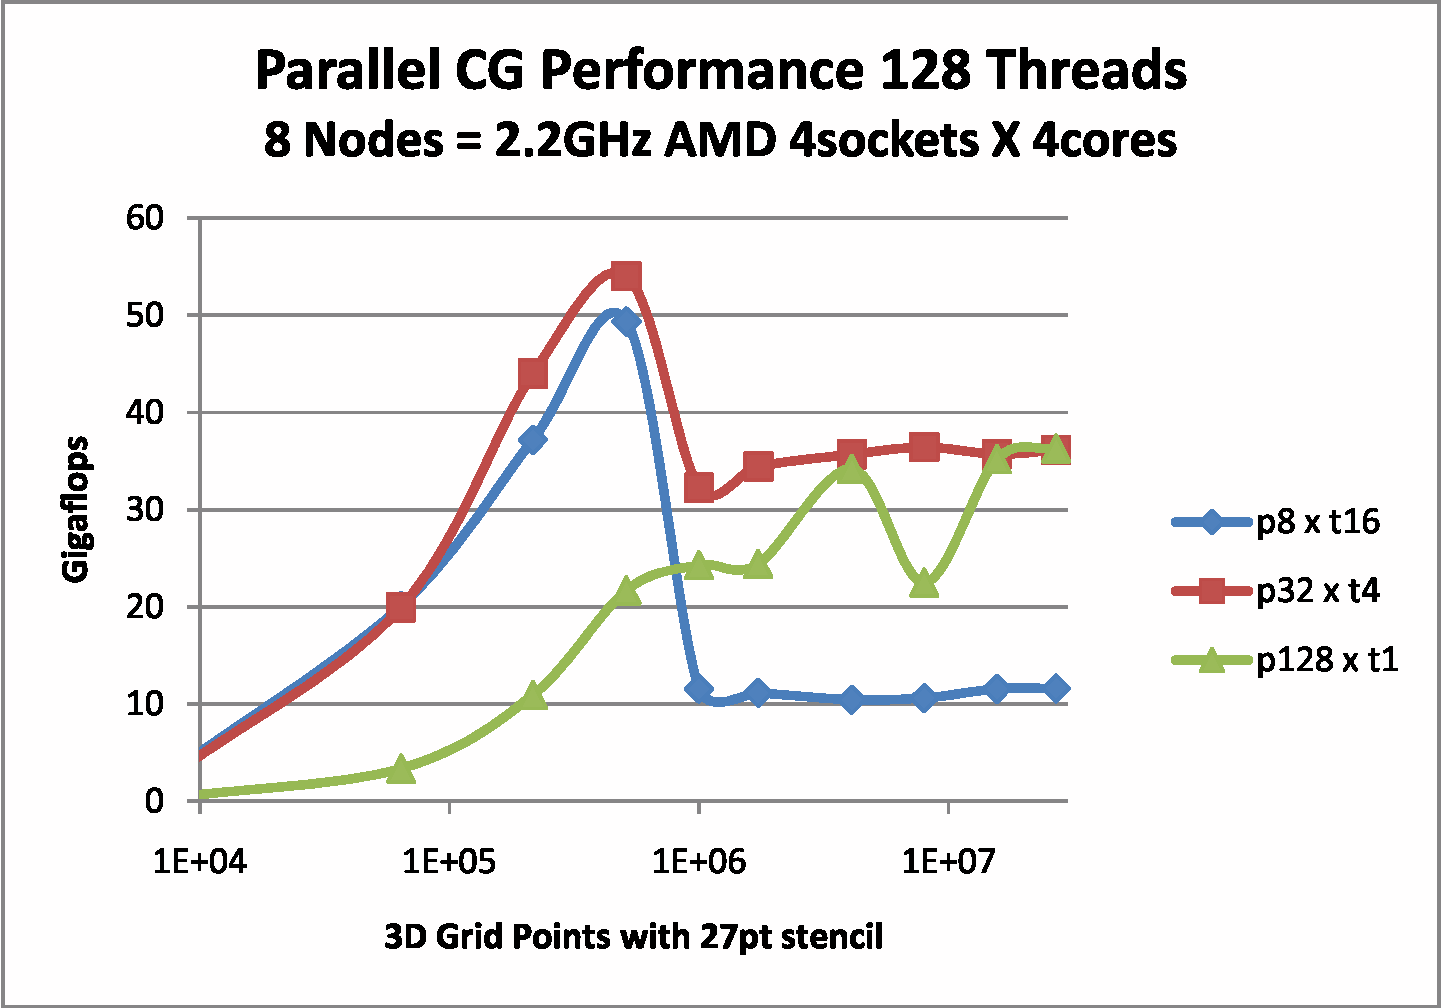
\includegraphics[viewport=1in 0.5in 8.5in 6.5in,angle=0,scale=0.5]{figures/test-hhpccg-intel-11-1-mpi-exe-np8-no-overlap-2}
\caption{Comparison of hybrid parallel conjugate gradient iteration performance for 8 compute nodes with 128 threads: p8 x t16 = one MPI process per node, p32 x t4 = one MPI process per socket, and p128 x t1 = one MPI process per core.}
\label{fig:CGPerf:np8}
\end{figure}

\begin{figure}[h]
\center
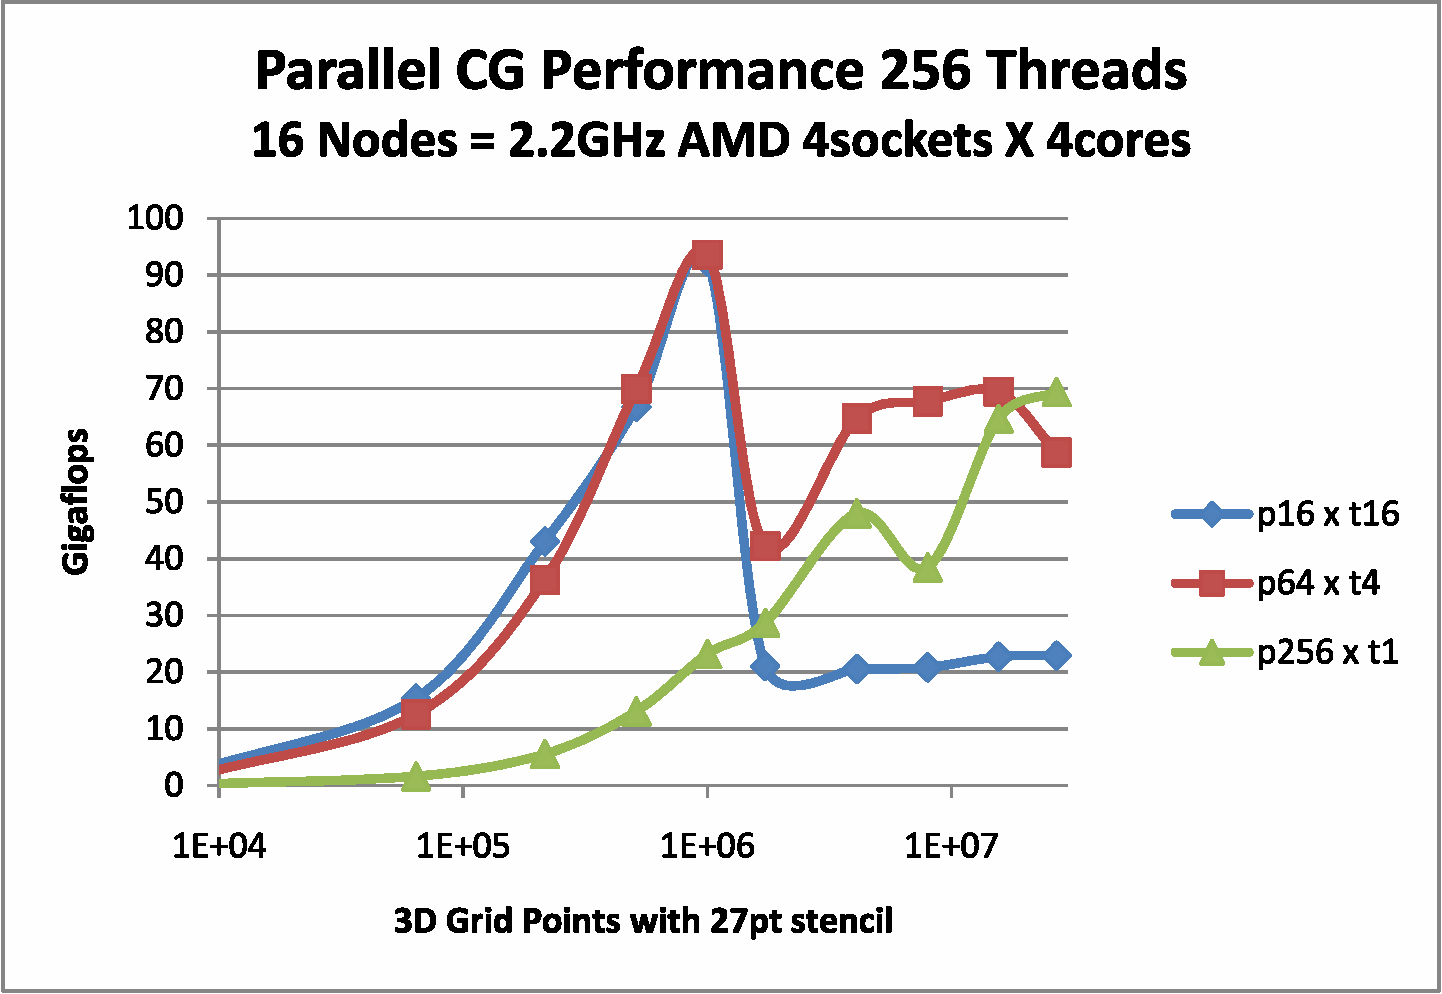
\includegraphics[viewport=1in 0.5in 8.5in 6.5in,angle=0,scale=0.5]{figures/test-hhpccg-intel-11-1-mpi-exe-np16-no-overlap-2}
\caption{Comparison of hybrid parallel conjugate gradient iteration performance for 16 compute nodes with 256 threads: p16 x t16 = one MPI process per node, p64 x t4 = one MPI process per socket, and p256 x t1 = one MPI process per core.}
\label{fig:CGPerf:np16}
\end{figure}

\begin{figure}[h]
\center
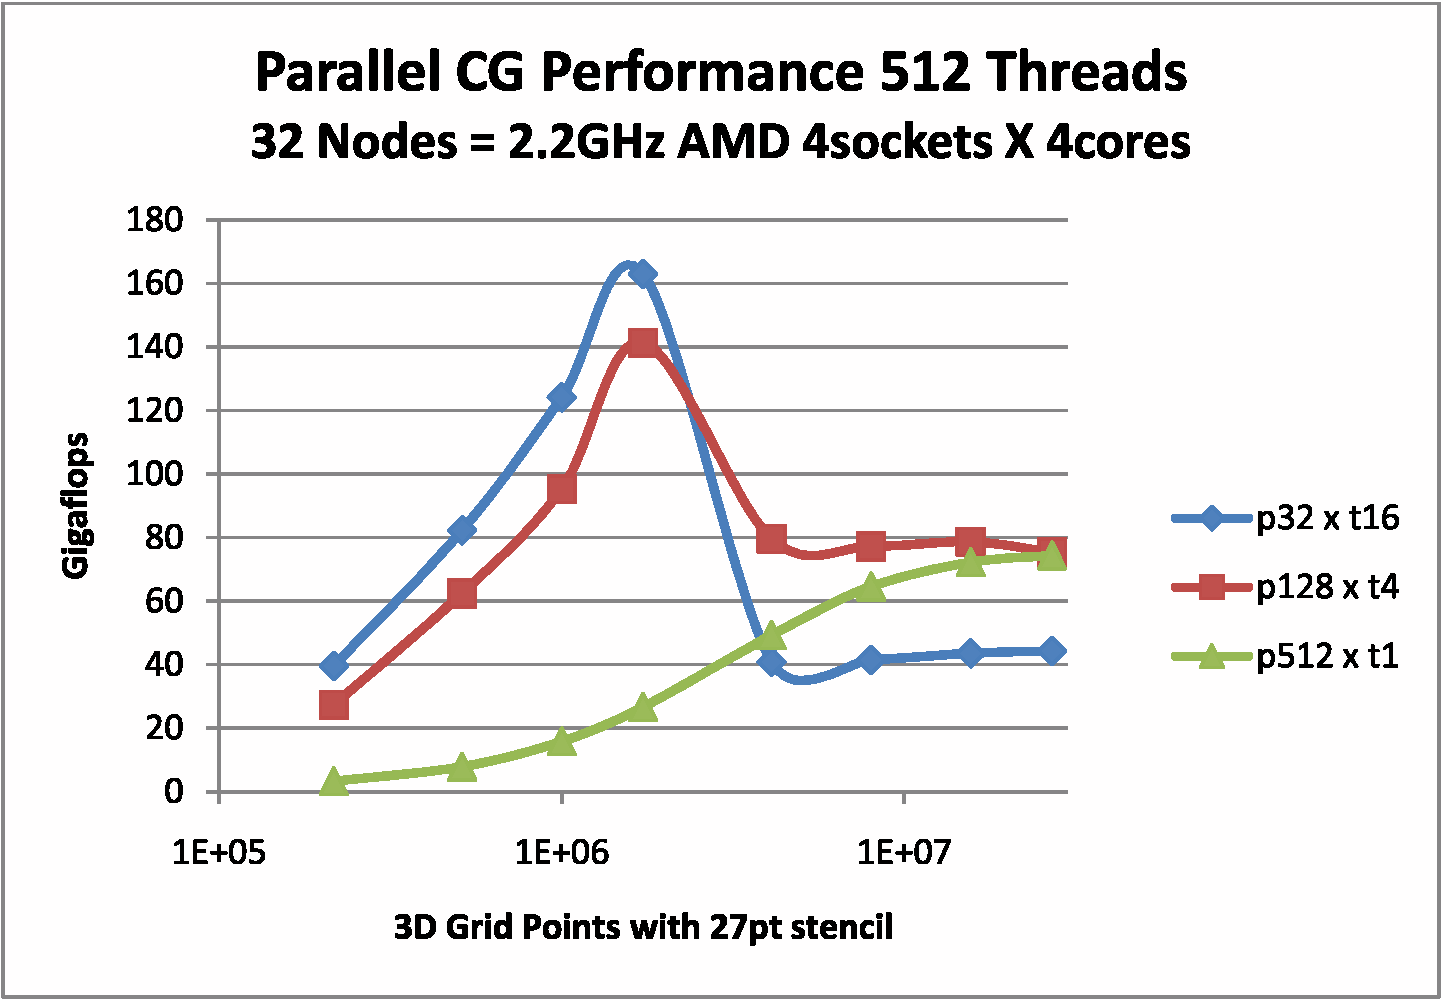
\includegraphics[viewport=1in 0.5in 8.5in 6.5in,angle=0,scale=0.5]{figures/test-hhpccg-intel-11-1-mpi-exe-np32-no-overlap}
\caption{Comparison of hybrid parallel conjugate gradient iteration performance for 32 compute nodes with 512 threads: p32 x t16 = one MPI process per node, p128 x t4 = one MPI process per socket, and p512 x t1 = one MPI process per core.}
\label{fig:CGPerf:np32}
\end{figure}


\begin{figure}[h]
\center
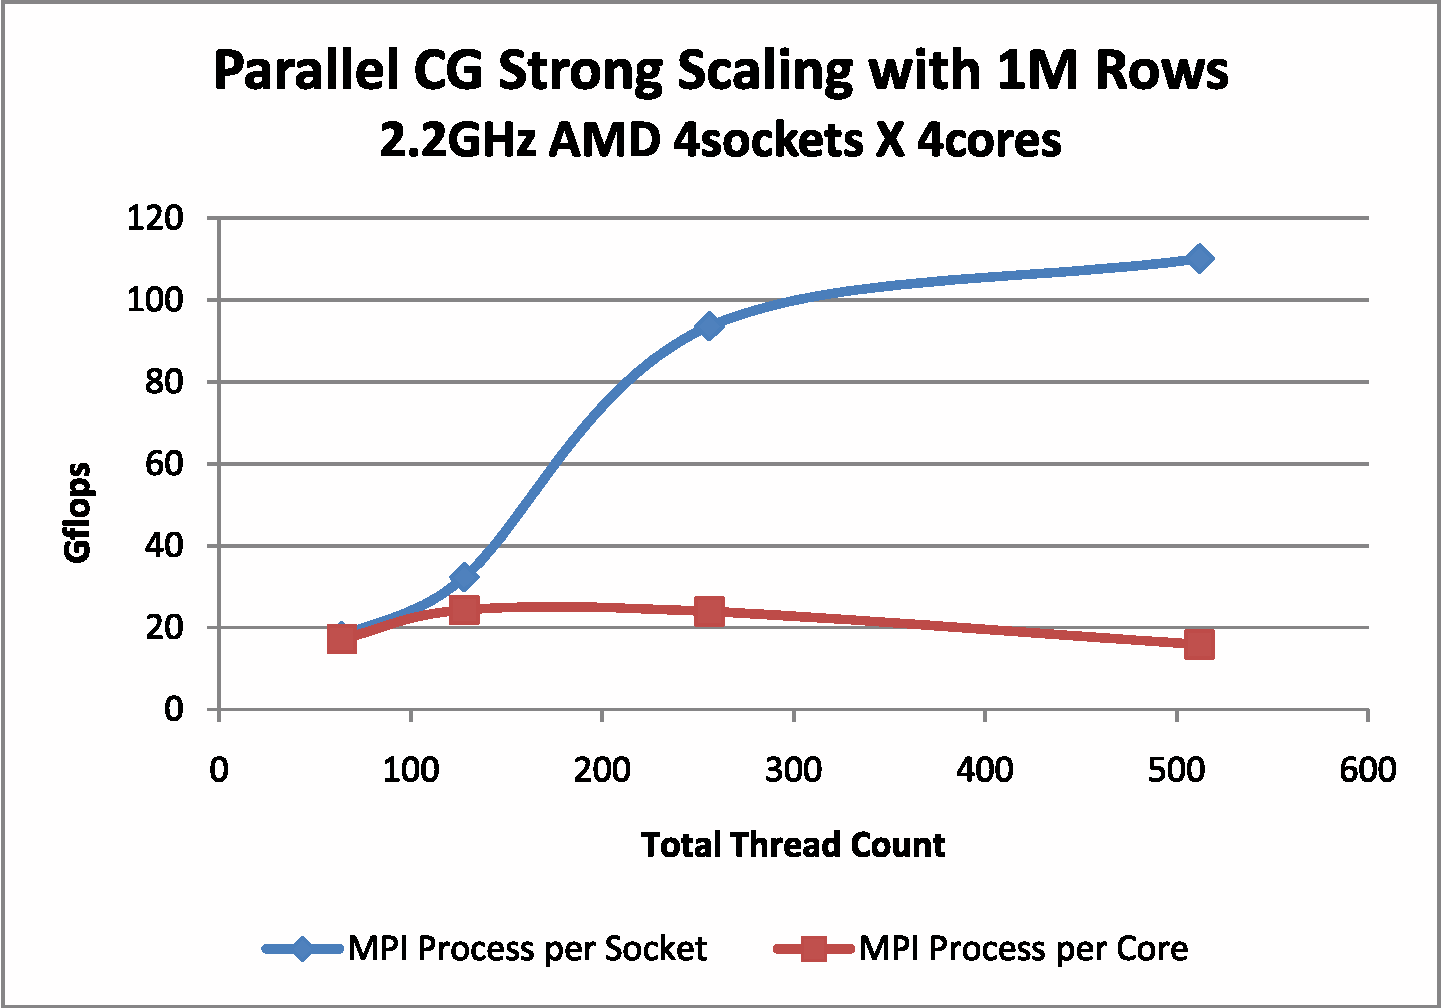
\includegraphics[viewport=1in 0.5in 8.5in 6.5in,angle=0,scale=0.5]{figures/StrongScaling1000k}
\caption{Hybrid parallel conjugate gradient iteration strong scaling for 1M rows: one MPI process with 4 threads per CPU socket versus one MPI process per CPU core.}
\label{fig:CGPerf:scaling1M}
\end{figure}

\begin{figure}[h]
\center
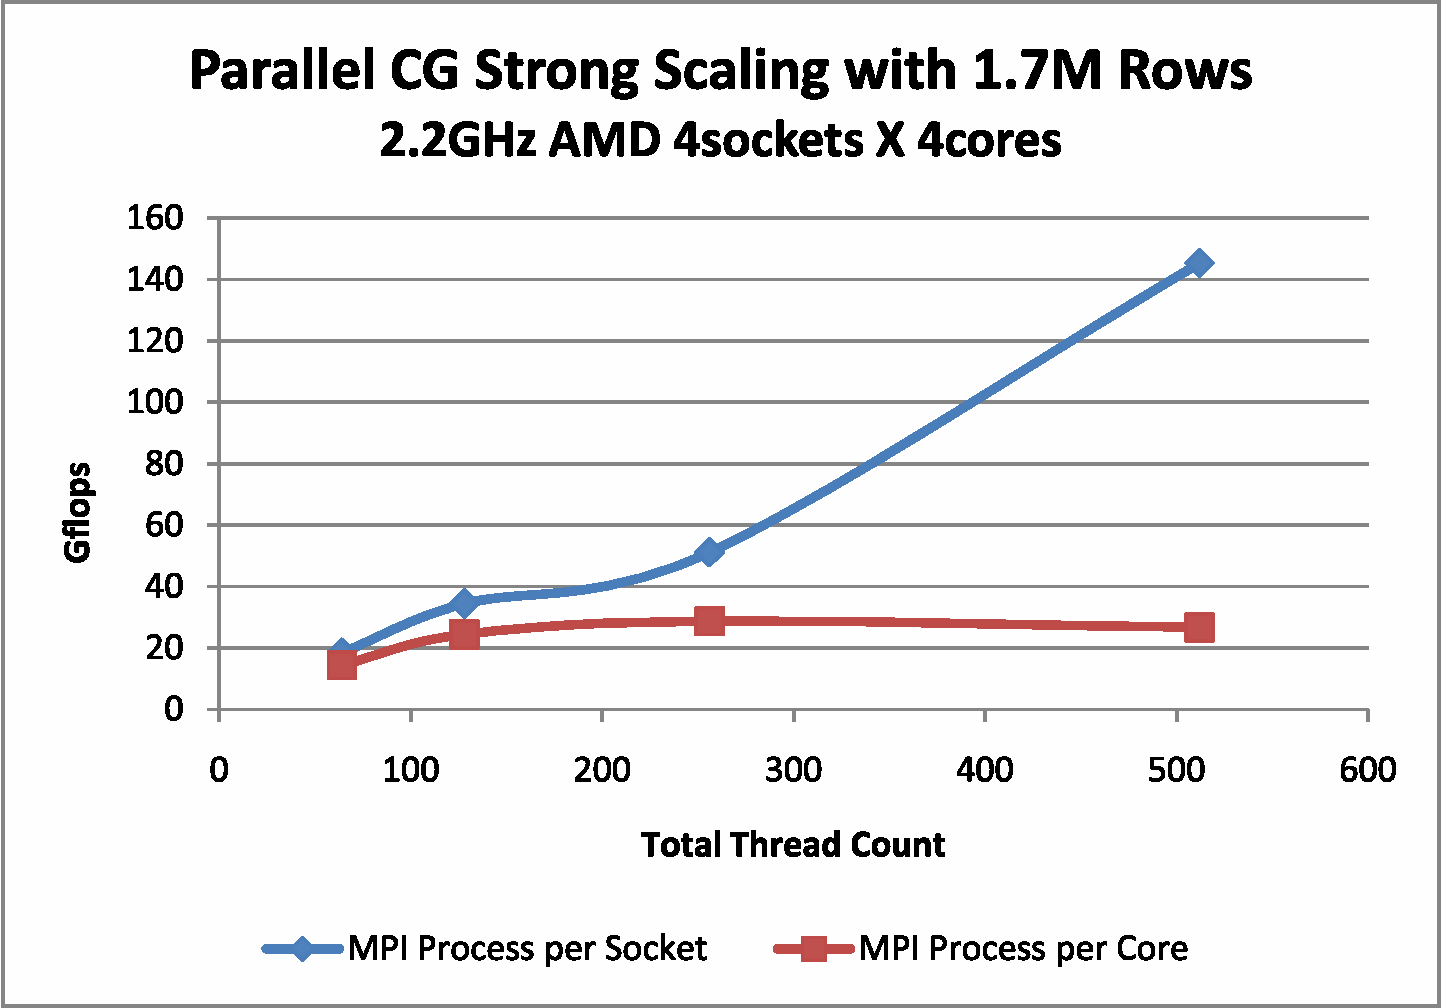
\includegraphics[viewport=1in 0.5in 8.5in 6.5in,angle=0,scale=0.5]{figures/StrongScaling1700k}
\caption{Hybrid parallel conjugate gradient iteration strong scaling for 1.7M rows: one MPI process with 4 threads per CPU socket versus one MPI process per CPU core.}
\label{fig:CGPerf:scaling1.7M}
\end{figure}


\begin{figure}[h]
\center
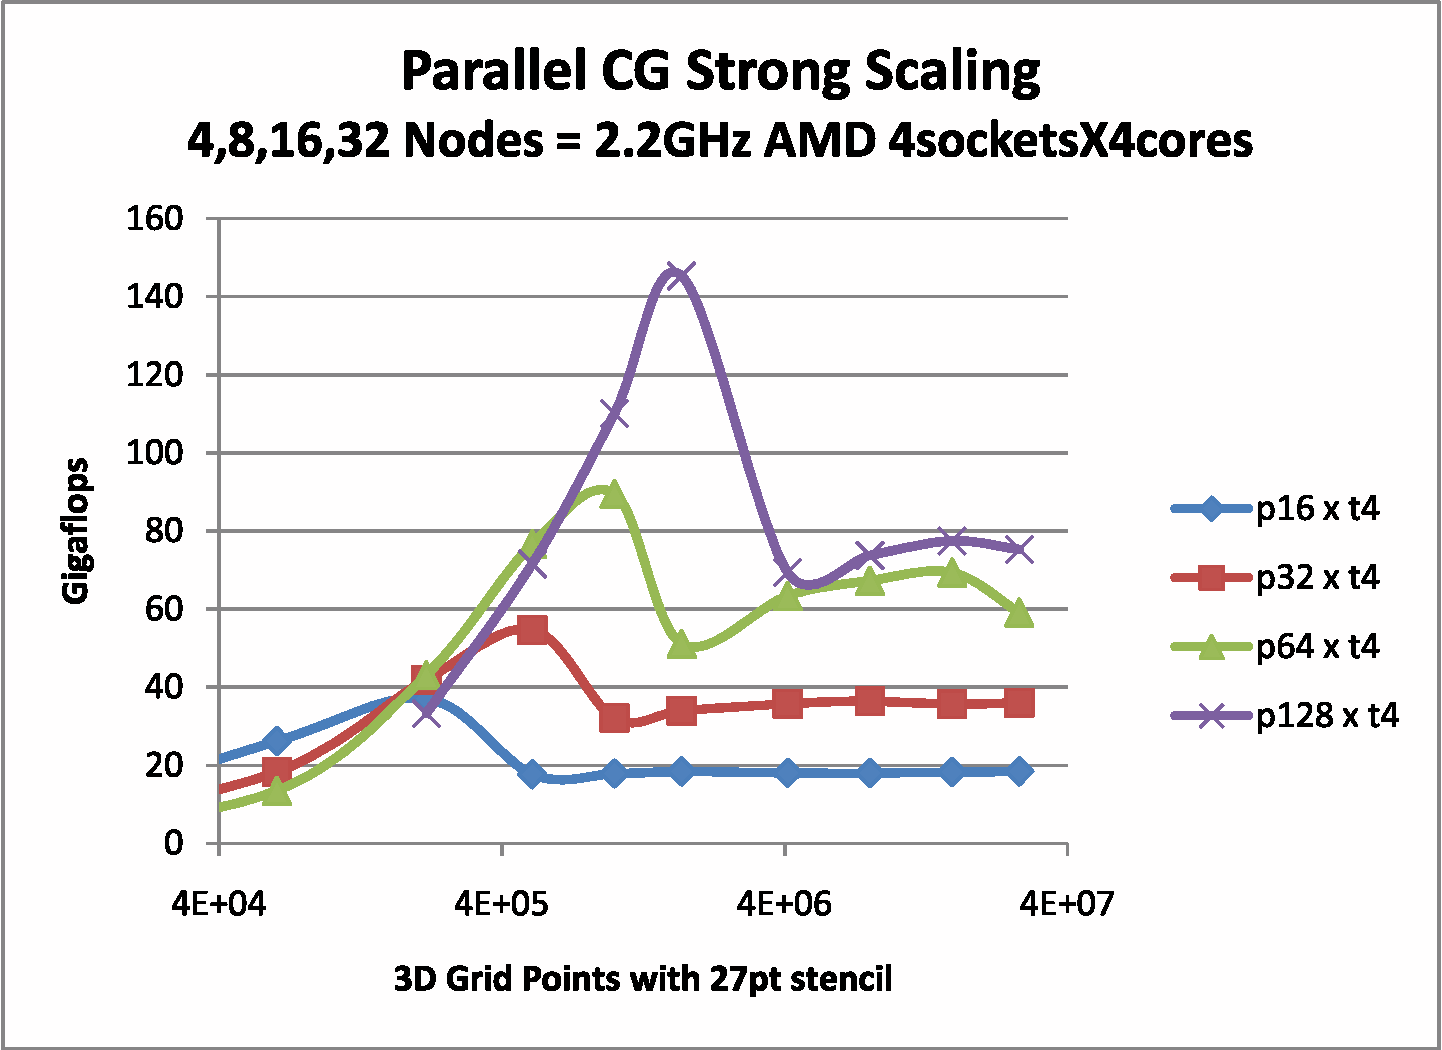
\includegraphics[viewport=1in 0.5in 8.5in 6.5in,angle=0,scale=0.5]{figures/test-hhpccg-intel-11-1-mpi-exe-scaling-no-overlap-2}
\caption{Hybrid parallel conjugate gradient iteration strong scaling with one MPI process and 4 threads per CPU socket.  Strong scaling over 64, 128, 256, and 512 threads is observed for a range of problem sizes by noting the associated problem-size point on each curve.}
\label{fig:CGPerf:scaling}
\end{figure}


\clearpage

\subsubsection{Fused Parallel Kernels}

Thread-parallel performance is most significantly improved by fused parallel kernels,
as per Algorithms~\ref{alg:CG-fused}~and~\ref{alg:FusedMXV},
when thread start/completion overhead is costly compare to kernel's computational costs.
%
This result can be seen in Figures~\ref{fig:CGPerf:np4:fusing}~and~\ref{fig:CGPerf:np32:fusing},
where CG iteration performance improvements are greater for small matrices than for larger matrices.
%
In these graphs the speed up is computed as the performance difference between the fused parallel kernel and conventional parallel kernel implementations, divided by the performance of the conventional parallel kernel implementation.


\begin{figure}[h]
\center
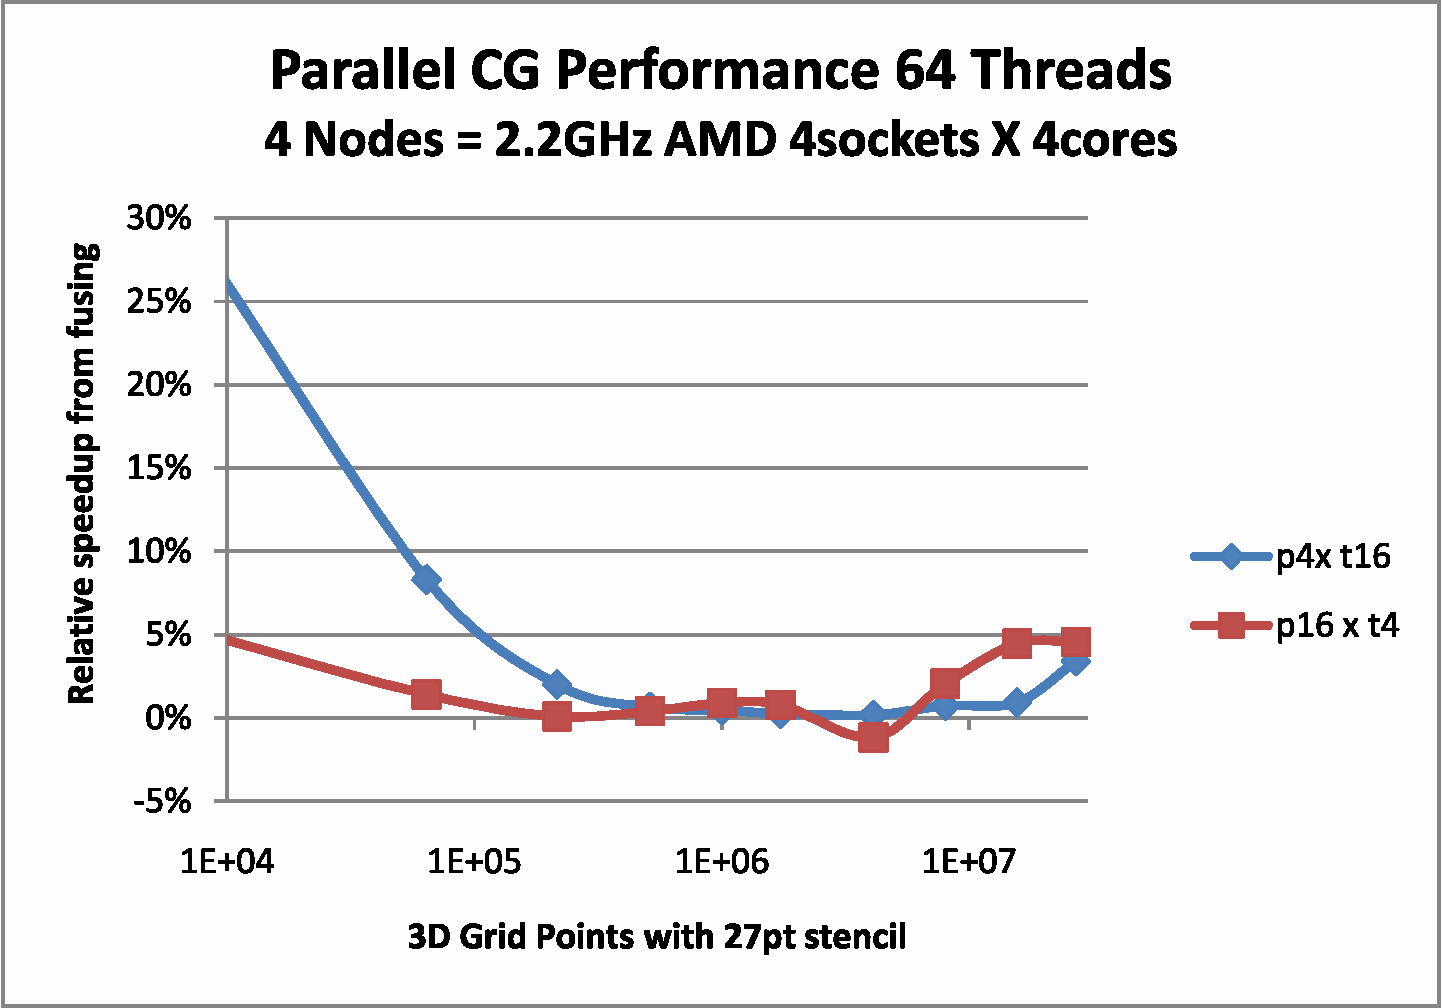
\includegraphics[viewport=1in 0.5in 8.5in 7in,angle=0,scale=0.5]{figures/test-hhpccg-intel-11-1-mpi-exe-np4-no-overlap-fusing}
\caption{Hybrid parallel conjugate gradient iteration relative performance improvement for parallel fused kernels with 4 compute nodes and 64 threads: p4 x t16 = one MPI process per node and p16 x t4 = one MPI process per socket.}
\label{fig:CGPerf:np4:fusing}
\end{figure}

\begin{figure}[h]
\center
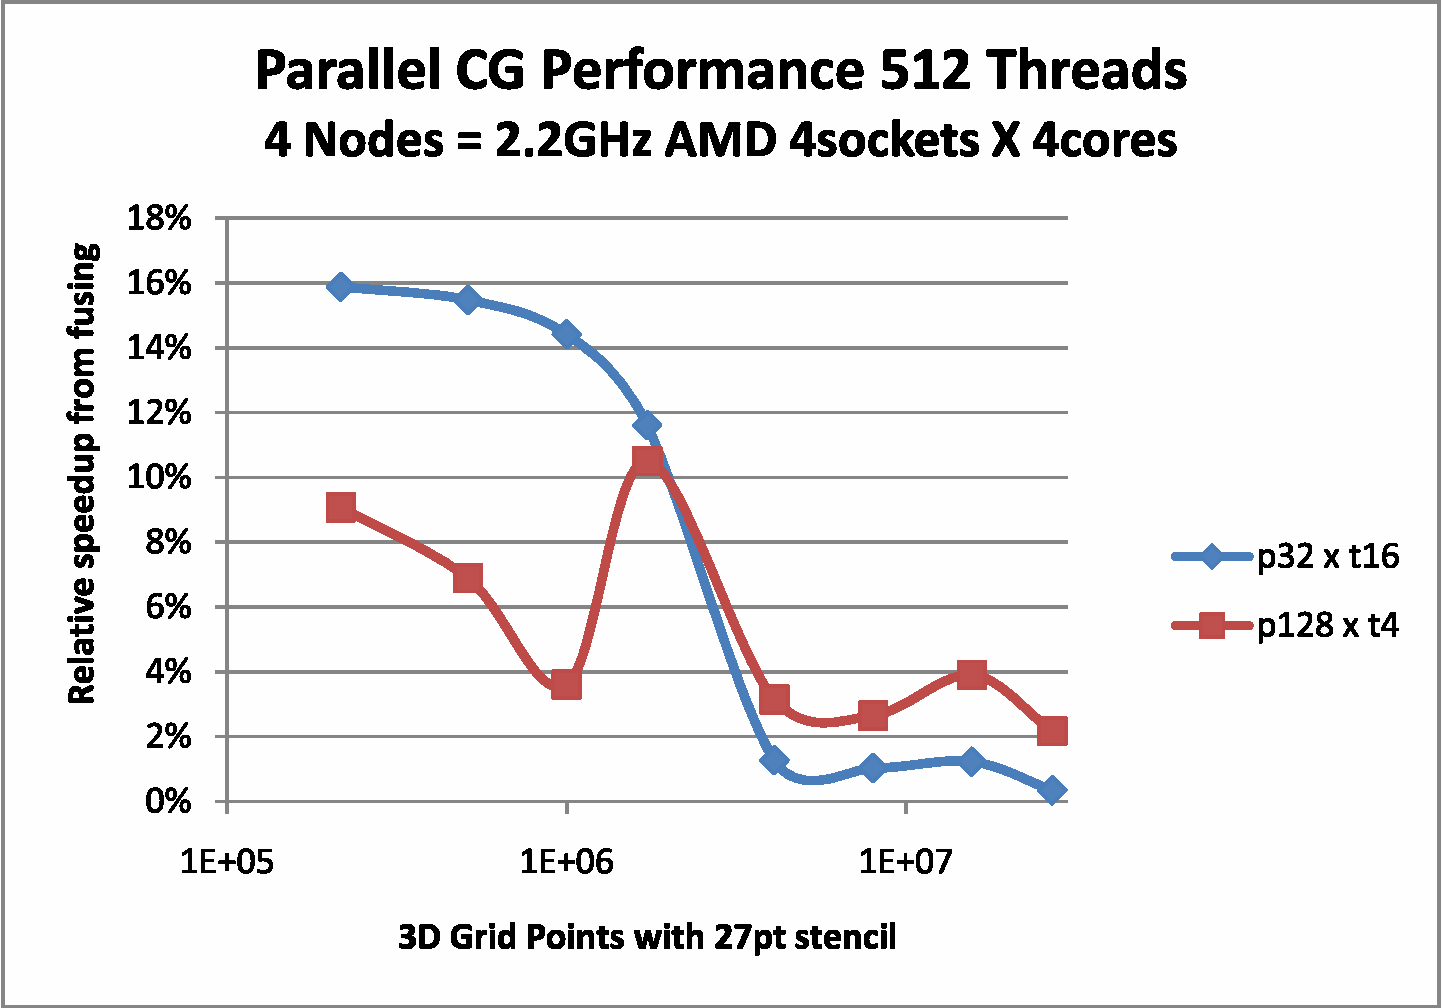
\includegraphics[viewport=1in 0.5in 8.5in 7in,angle=0,scale=0.5]{figures/test-hhpccg-intel-11-1-mpi-exe-np32-no-overlap-fusing}
\caption{Hybrid parallel conjugate gradient iteration relative performance improvement for parallel fused kernels with 32 compute nodes and 512 threads: p32 x t16 = one MPI process per node and p128 x t4 = one MPI process per socket.}
\label{fig:CGPerf:np32:fusing}
\end{figure}

















\section{Conclusion}

The ThreadPool library within Trilinos provides a simple, minimalistic API for HPC applications to effectively use hybrid parallelism on HPC systems with CPU-based manycore nodes.
%
The ThreadPool library is currently implemented in the standard C language using the standard \textbf{pthread} library.
%
The ThreadPool library creates a pool of \emph{worker} threads which are held ready for use by the application.
%
The ThreadPool API assumes an application programming model
(Figure~\ref{fig:HybridParallelArchitecture}) which separates its software into lower-level stateless computational kernels and higher-level control flow and resource management components.
%
ThreadPool functions are called by an application to run computational kernels thread-parallel.
%
Inter-thread synchronization is supported through mutually exclusive execution locks, or through more efficient reduction operations.



A simple mini-application performing conjugate gradient solution algorithm iterations was run on Sandia National Laboratories' \emph{glory} cluster with 272 quad-socket / quad-core compute nodes with non-uniform memory access (NUMA).
%
This mini-application on this cluster demonstrated significantly improved performance, for CPU cache-resident problems, by nesting thread-parallelism within CPU-cores, while retaining MPI-parallelism between CPU-sockets.
%
For large problems with performance limited by access to main memory the performance improvement is relatively small.
%
These results show that hybrid thread-parallelism nested within MPI-parallelism can improve HPC application performance when run on clusters of multicore compute nodes.



\subsection{To-be-done: Comparison other Threading Capabilities}

Hybrid parallel performance results presented in this report use standard pthreads managed by the ThreadPool interface.
%
Other thread parallel mechanisms such as OpenMP and TBB could yield different performance results.
%
The hybrid parallel conjugate gradient performance test cases could be re-implemented using OpenMP and TBB to compare and evaluate the ThreadPool library's efficiency and API compared to these other threading capabilities.



 


%----------------------------------------------------------------------%

\bibliographystyle{plain}
\bibliography{References}  

%----------------------------------------------------------------------%

\begin{SANDdistribution}[NM]
    % Housekeeping copies necessary for every unclassified report:
    % \SANDdistCRADA	% If this report is about CRADA work
    % \SANDdistPatent	% If this report has a Patent Caution or Patent Interest
    % \SANDdistLDRD	% If this report is about LDRD work

    % Some external Addresses
    %\SANDdistExternal{1}{An Address\\ 99 $99^{th}$ street NW\\City, State}
    %\SANDdistExternal{3}{Some Address\\ and street\\City, State}
    %\SANDdistExternal{12}{Another Address\\ On a street\\City, State\\U.S.A.}
    %\bigskip


    % The following MUST BE between the external and internal distributions!
    % \SANDdistClassified % If this report is classified


    % Internal Addresses
    \SANDdistInternal{1}{0380}{David E. Womble}{01540}
    \SANDdistInternal{1}{0832}{Ted D. Blacker}{01543}
    \SANDdistInternal{1}{0382}{H. Carter Edwards}{01543}
    \SANDdistInternal{1}{0382}{Michael W. Glass}{01543}
    \SANDdistInternal{1}{0382}{Alan B. Williams}{01543}
    \SANDdistInternal{1}{1320}{S. Scott Collis}{01416}
    \SANDdistInternal{1}{1320}{Michael Heroux}{01416}


    % Example of a mail channel use (instead of a mail stop)
    %\SANDdistInternalM{1}{M9999}{Someone}{01234}

\end{SANDdistribution}

\end{document}
